\documentclass{standalone}
\usepackage{tikz}
\usetikzlibrary{patterns, positioning}
\usepackage[sfdefault]{ClearSans} %% option 'sfdefault' activates Clear Sans as the default text font
\usepackage[T1]{fontenc}

\begin{document}
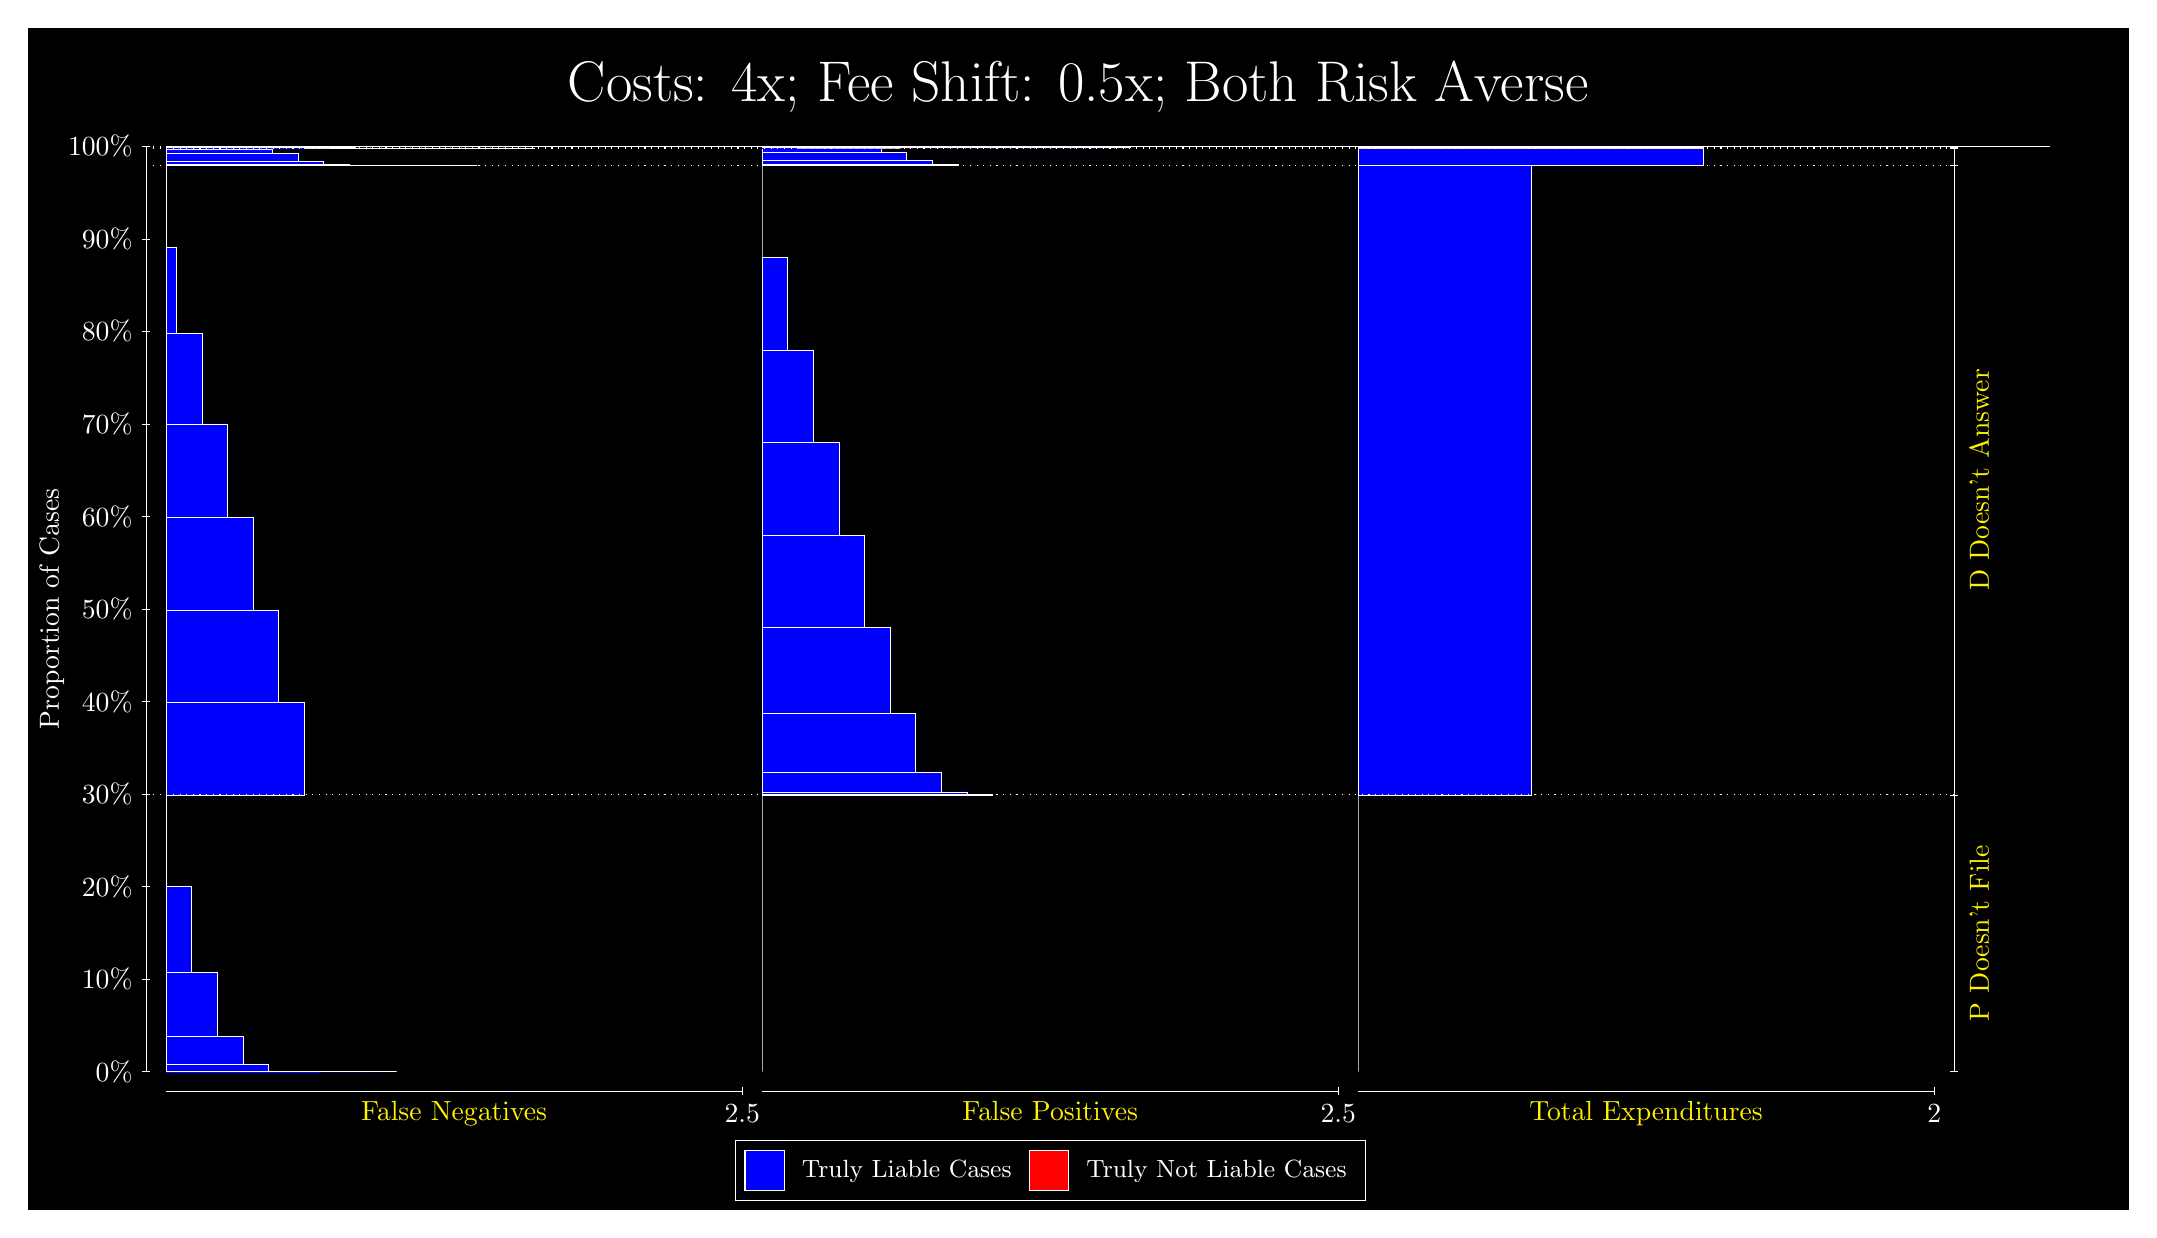
\begin{tikzpicture}
\draw[fill=black] (0,0) rectangle (26.667,15);
\draw[text=white] (0,13.5) rectangle (26.667,15) node[midway] {\huge Costs: 4x; Fee Shift: 0.5x; Both Risk Averse};
\draw[white, very thin] (1.5,1.75) -- (1.5,13.5);
\node[rotate=90, text=white, anchor=center] at (0.3, 7.625) {Proportion of Cases};
\draw[white, very thin] (1.45,1.75) -- (1.55,1.75);
\node[text=white, anchor=east] at (1.45, 1.75) {0\%};
\draw[white, very thin] (1.45,2.925) -- (1.55,2.925);
\node[text=white, anchor=east] at (1.45, 2.925) {10\%};
\draw[white, very thin] (1.45,4.1) -- (1.55,4.1);
\node[text=white, anchor=east] at (1.45, 4.1) {20\%};
\draw[white, very thin] (1.45,5.275) -- (1.55,5.275);
\node[text=white, anchor=east] at (1.45, 5.275) {30\%};
\draw[white, very thin] (1.45,6.45) -- (1.55,6.45);
\node[text=white, anchor=east] at (1.45, 6.45) {40\%};
\draw[white, very thin] (1.45,7.625) -- (1.55,7.625);
\node[text=white, anchor=east] at (1.45, 7.625) {50\%};
\draw[white, very thin] (1.45,8.8) -- (1.55,8.8);
\node[text=white, anchor=east] at (1.45, 8.8) {60\%};
\draw[white, very thin] (1.45,9.975) -- (1.55,9.975);
\node[text=white, anchor=east] at (1.45, 9.975) {70\%};
\draw[white, very thin] (1.45,11.15) -- (1.55,11.15);
\node[text=white, anchor=east] at (1.45, 11.15) {80\%};
\draw[white, very thin] (1.45,12.325) -- (1.55,12.325);
\node[text=white, anchor=east] at (1.45, 12.325) {90\%};
\draw[white, very thin] (1.45,13.5) -- (1.55,13.5);
\node[text=white, anchor=east] at (1.45, 13.5) {100\%};

\draw[white, very thin] (24.457,1.75) -- (24.457,13.5);
\draw[white, very thin] (24.407,1.75) -- (24.507,1.75);
\node[anchor=west] at (24.407, 1.75) {};
\draw[white, very thin] (24.407,5.264) -- (24.507,5.264);
\node[anchor=west] at (24.407, 5.264) {};
\draw[white, very thin] (24.407,13.262) -- (24.507,13.262);
\node[anchor=west] at (24.407, 13.262) {};
\draw[white, very thin] (24.407,13.476) -- (24.507,13.476);
\node[anchor=west] at (24.407, 13.476) {};
\draw[white, very thin] (24.407,13.484) -- (24.507,13.484);
\node[anchor=west] at (24.407, 13.484) {};
\draw[white, very thin] (24.407,13.499) -- (24.507,13.499);
\node[anchor=west] at (24.407, 13.499) {};
\draw[white, very thin] (24.407,13.5) -- (24.507,13.5);
\node[anchor=west] at (24.407, 13.5) {};

\draw[white, very thin, fill=blue] (1.75,1.75) rectangle (4.6775,1.75);
\draw[white, very thin, fill=blue] (1.75,1.75) rectangle (4.3523,1.75);
\draw[white, very thin, fill=blue] (1.75,1.75) rectangle (4.027,1.75);
\draw[white, very thin, fill=blue] (1.75,1.75) rectangle (3.7017,1.7503);
\draw[white, very thin, fill=blue] (1.75,1.7503) rectangle (3.3764,1.7576);
\draw[white, very thin, fill=blue] (1.75,1.7576) rectangle (3.0511,1.8361);
\draw[white, very thin, fill=blue] (1.75,1.8361) rectangle (2.7258,2.1984);
\draw[white, very thin, fill=blue] (1.75,2.1984) rectangle (2.4006,3.0086);
\draw[white, very thin, fill=blue] (1.75,3.0086) rectangle (2.0753,4.0995);
\draw[white, very thin, fill=red] (1.75,4.0995) rectangle (1.75,4.0995);
\draw[white, very thin, fill=blue] (1.75,4.0995) rectangle (1.75,5.264);
\draw[white, very thin, fill=blue] (1.75,5.264) rectangle (3.5065,6.439);
\draw[white, very thin, fill=blue] (1.75,6.439) rectangle (3.1812,7.614);
\draw[white, very thin, fill=blue] (1.75,7.614) rectangle (2.856,8.789);
\draw[white, very thin, fill=blue] (1.75,8.789) rectangle (2.5307,9.9637);
\draw[white, very thin, fill=blue] (1.75,9.9637) rectangle (2.2054,11.131);
\draw[white, very thin, fill=blue] (1.75,11.131) rectangle (1.8801,12.221);
\draw[white, very thin, fill=red] (1.75,12.221) rectangle (1.75,12.221);
\draw[white, very thin, fill=blue] (1.75,12.221) rectangle (1.75,13.262);
\draw[white, very thin, fill=blue] (1.75,13.262) rectangle (5.7022,13.262);
\draw[white, very thin, fill=blue] (1.75,13.262) rectangle (5.3769,13.262);
\draw[white, very thin, fill=blue] (1.75,13.262) rectangle (5.0516,13.262);
\draw[white, very thin, fill=blue] (1.75,13.262) rectangle (4.7263,13.262);
\draw[white, very thin, fill=blue] (1.75,13.262) rectangle (4.4011,13.262);
\draw[white, very thin, fill=blue] (1.75,13.262) rectangle (4.0758,13.266);
\draw[white, very thin, fill=blue] (1.75,13.266) rectangle (3.7505,13.309);
\draw[white, very thin, fill=blue] (1.75,13.309) rectangle (3.4252,13.412);
\draw[white, very thin, fill=blue] (1.75,13.412) rectangle (3.0999,13.467);
\draw[white, very thin, fill=blue] (1.75,13.467) rectangle (2.7746,13.476);
\draw[white, very thin, fill=red] (1.75,13.476) rectangle (1.75,13.476);
\draw[white, very thin, fill=blue] (1.75,13.476) rectangle (6.4341,13.476);
\draw[white, very thin, fill=blue] (1.75,13.476) rectangle (6.1088,13.476);
\draw[white, very thin, fill=blue] (1.75,13.476) rectangle (5.7835,13.476);
\draw[white, very thin, fill=blue] (1.75,13.476) rectangle (5.4582,13.476);
\draw[white, very thin, fill=blue] (1.75,13.476) rectangle (5.1329,13.476);
\draw[white, very thin, fill=blue] (1.75,13.476) rectangle (4.8077,13.476);
\draw[white, very thin, fill=blue] (1.75,13.476) rectangle (4.4824,13.479);
\draw[white, very thin, fill=blue] (1.75,13.479) rectangle (4.1571,13.483);
\draw[white, very thin, fill=blue] (1.75,13.483) rectangle (3.8318,13.483);
\draw[white, very thin, fill=blue] (1.75,13.483) rectangle (3.5065,13.484);
\draw[white, very thin, fill=red] (1.75,13.484) rectangle (1.75,13.484);
\draw[white, very thin, fill=blue] (1.75,13.484) rectangle (3.5065,13.484);
\draw[white, very thin, fill=blue] (1.75,13.484) rectangle (3.1812,13.484);
\draw[white, very thin, fill=blue] (1.75,13.484) rectangle (2.856,13.484);
\draw[white, very thin, fill=blue] (1.75,13.484) rectangle (2.5307,13.484);
\draw[white, very thin, fill=blue] (1.75,13.484) rectangle (2.2054,13.484);
\draw[white, very thin, fill=blue] (1.75,13.484) rectangle (1.8801,13.486);
\draw[white, very thin, fill=red] (1.75,13.486) rectangle (1.75,13.486);
\draw[white, very thin, fill=blue] (1.75,13.486) rectangle (1.75,13.499);
\draw[white, very thin, fill=blue] (1.75,13.499) rectangle (9.9471,13.499);
\draw[white, very thin, fill=blue] (1.75,13.499) rectangle (9.6218,13.499);
\draw[white, very thin, fill=blue] (1.75,13.499) rectangle (9.2966,13.499);
\draw[white, very thin, fill=blue] (1.75,13.499) rectangle (8.9713,13.499);
\draw[white, very thin, fill=blue] (1.75,13.499) rectangle (8.646,13.499);
\draw[white, very thin, fill=blue] (1.75,13.499) rectangle (8.3207,13.499);
\draw[white, very thin, fill=blue] (1.75,13.499) rectangle (8.3207,13.499);
\draw[white, very thin, fill=blue] (1.75,13.499) rectangle (7.9954,13.499);
\draw[white, very thin, fill=blue] (1.75,13.499) rectangle (7.9954,13.499);
\draw[white, very thin, fill=blue] (1.75,13.499) rectangle (7.6702,13.5);
\draw[white, very thin, fill=blue] (1.75,13.5) rectangle (7.3449,13.5);
\draw[white, very thin, fill=blue] (1.75,13.5) rectangle (7.3449,13.5);
\draw[white, very thin, fill=blue] (1.75,13.5) rectangle (7.0196,13.5);
\draw[white, very thin, fill=blue] (1.75,13.5) rectangle (6.6943,13.5);
\draw[white, very thin, fill=blue] (1.75,13.5) rectangle (6.369,13.5);
\draw[white, very thin, fill=blue] (1.75,13.5) rectangle (5.4582,13.5);
\draw[white, very thin, fill=blue] (1.75,13.5) rectangle (5.1329,13.5);
\draw[white, very thin, fill=blue] (1.75,13.5) rectangle (4.8077,13.5);
\draw[white, very thin, fill=blue] (1.75,13.5) rectangle (4.8077,13.5);
\draw[white, very thin, fill=blue] (1.75,13.5) rectangle (4.4824,13.5);
\draw[white, very thin, fill=blue] (1.75,13.5) rectangle (4.4824,13.5);
\draw[white, very thin, fill=blue] (1.75,13.5) rectangle (4.1571,13.5);
\draw[white, very thin, fill=blue] (1.75,13.5) rectangle (3.8318,13.5);
\draw[white, very thin, fill=blue] (1.75,13.5) rectangle (3.8318,13.5);
\draw[white, very thin, fill=blue] (1.75,13.5) rectangle (3.5065,13.5);
\draw[white, very thin, fill=blue] (1.75,13.5) rectangle (3.1812,13.5);
\draw[white, very thin, fill=blue] (1.75,13.5) rectangle (3.1812,13.5);
\draw[white, very thin, fill=blue] (1.75,13.5) rectangle (3.1812,13.5);
\draw[white, very thin, fill=blue] (1.75,13.5) rectangle (2.856,13.5);
\draw[white, very thin, fill=blue] (1.75,13.5) rectangle (2.856,13.5);
\draw[white, very thin, fill=blue] (1.75,13.5) rectangle (2.5307,13.5);
\draw[white, very thin, fill=blue] (1.75,13.5) rectangle (2.5307,13.5);
\draw[white, very thin, fill=blue] (1.75,13.5) rectangle (2.5307,13.5);
\draw[white, very thin, fill=blue] (1.75,13.5) rectangle (2.2054,13.5);
\draw[white, very thin, fill=blue] (1.75,13.5) rectangle (2.2054,13.5);
\draw[white, very thin, fill=blue] (1.75,13.5) rectangle (1.8801,13.5);
\draw[white, very thin, fill=blue] (1.75,13.5) rectangle (1.8801,13.5);
\draw[white, very thin, fill=red] (1.75,13.5) rectangle (1.75,13.5);
\draw[white, very thin, fill=blue] (1.75,13.5) rectangle (1.75,13.5);
\draw[white, very thin, fill=red] (9.3189,1.75) rectangle (9.3189,1.75);
\draw[white, very thin, fill=blue] (9.3189,1.75) rectangle (9.3189,5.264);
\draw[white, very thin, fill=red] (9.3189,5.264) rectangle (12.246,5.264);
\draw[white, very thin, fill=blue] (9.3189,5.264) rectangle (12.246,5.265);
\draw[white, very thin, fill=blue] (9.3189,5.265) rectangle (11.921,5.2928);
\draw[white, very thin, fill=blue] (9.3189,5.2928) rectangle (11.596,5.5466);
\draw[white, very thin, fill=blue] (9.3189,5.5466) rectangle (11.271,6.3052);
\draw[white, very thin, fill=blue] (9.3189,6.3052) rectangle (10.945,7.3948);
\draw[white, very thin, fill=blue] (9.3189,7.3948) rectangle (10.62,8.5623);
\draw[white, very thin, fill=blue] (9.3189,8.5623) rectangle (10.295,9.737);
\draw[white, very thin, fill=blue] (9.3189,9.737) rectangle (9.9694,10.912);
\draw[white, very thin, fill=blue] (9.3189,10.912) rectangle (9.6442,12.087);
\draw[white, very thin, fill=blue] (9.3189,12.087) rectangle (9.3189,13.262);
\draw[white, very thin, fill=red] (9.3189,13.262) rectangle (11.807,13.262);
\draw[white, very thin, fill=blue] (9.3189,13.262) rectangle (11.807,13.271);
\draw[white, very thin, fill=blue] (9.3189,13.271) rectangle (11.482,13.326);
\draw[white, very thin, fill=blue] (9.3189,13.326) rectangle (11.157,13.429);
\draw[white, very thin, fill=blue] (9.3189,13.429) rectangle (10.831,13.472);
\draw[white, very thin, fill=blue] (9.3189,13.472) rectangle (10.506,13.476);
\draw[white, very thin, fill=blue] (9.3189,13.476) rectangle (10.181,13.476);
\draw[white, very thin, fill=blue] (9.3189,13.476) rectangle (9.8556,13.476);
\draw[white, very thin, fill=blue] (9.3189,13.476) rectangle (9.5303,13.476);
\draw[white, very thin, fill=blue] (9.3189,13.476) rectangle (9.3189,13.476);
\draw[white, very thin, fill=red] (9.3189,13.476) rectangle (11.075,13.476);
\draw[white, very thin, fill=blue] (9.3189,13.476) rectangle (11.075,13.476);
\draw[white, very thin, fill=blue] (9.3189,13.476) rectangle (10.75,13.477);
\draw[white, very thin, fill=blue] (9.3189,13.477) rectangle (10.425,13.48);
\draw[white, very thin, fill=blue] (9.3189,13.48) rectangle (10.1,13.483);
\draw[white, very thin, fill=blue] (9.3189,13.483) rectangle (9.7743,13.484);
\draw[white, very thin, fill=blue] (9.3189,13.484) rectangle (9.449,13.484);
\draw[white, very thin, fill=blue] (9.3189,13.484) rectangle (9.3189,13.484);
\draw[white, very thin, fill=red] (9.3189,13.484) rectangle (14.003,13.484);
\draw[white, very thin, fill=blue] (9.3189,13.484) rectangle (14.003,13.484);
\draw[white, very thin, fill=blue] (9.3189,13.484) rectangle (13.678,13.484);
\draw[white, very thin, fill=blue] (9.3189,13.484) rectangle (13.352,13.489);
\draw[white, very thin, fill=blue] (9.3189,13.489) rectangle (13.027,13.497);
\draw[white, very thin, fill=blue] (9.3189,13.497) rectangle (12.702,13.499);
\draw[white, very thin, fill=blue] (9.3189,13.499) rectangle (12.377,13.499);
\draw[white, very thin, fill=blue] (9.3189,13.499) rectangle (12.051,13.499);
\draw[white, very thin, fill=blue] (9.3189,13.499) rectangle (11.726,13.499);
\draw[white, very thin, fill=blue] (9.3189,13.499) rectangle (11.401,13.499);
\draw[white, very thin, fill=blue] (9.3189,13.499) rectangle (11.075,13.499);
\draw[white, very thin, fill=red] (9.3189,13.499) rectangle (17.516,13.499);
\draw[white, very thin, fill=blue] (9.3189,13.499) rectangle (17.516,13.499);
\draw[white, very thin, fill=red] (9.3189,13.499) rectangle (17.191,13.499);
\draw[white, very thin, fill=blue] (9.3189,13.499) rectangle (17.191,13.499);
\draw[white, very thin, fill=red] (9.3189,13.499) rectangle (16.865,13.499);
\draw[white, very thin, fill=blue] (9.3189,13.499) rectangle (16.865,13.499);
\draw[white, very thin, fill=red] (9.3189,13.499) rectangle (16.54,13.499);
\draw[white, very thin, fill=blue] (9.3189,13.499) rectangle (16.54,13.499);
\draw[white, very thin, fill=red] (9.3189,13.499) rectangle (16.215,13.499);
\draw[white, very thin, fill=blue] (9.3189,13.499) rectangle (16.215,13.499);
\draw[white, very thin, fill=red] (9.3189,13.499) rectangle (15.89,13.499);
\draw[white, very thin, fill=blue] (9.3189,13.499) rectangle (15.89,13.499);
\draw[white, very thin, fill=blue] (9.3189,13.499) rectangle (15.89,13.499);
\draw[white, very thin, fill=red] (9.3189,13.499) rectangle (15.564,13.499);
\draw[white, very thin, fill=blue] (9.3189,13.499) rectangle (15.564,13.499);
\draw[white, very thin, fill=blue] (9.3189,13.499) rectangle (15.564,13.499);
\draw[white, very thin, fill=blue] (9.3189,13.499) rectangle (15.239,13.5);
\draw[white, very thin, fill=blue] (9.3189,13.5) rectangle (15.239,13.5);
\draw[white, very thin, fill=blue] (9.3189,13.5) rectangle (14.914,13.5);
\draw[white, very thin, fill=blue] (9.3189,13.5) rectangle (14.914,13.5);
\draw[white, very thin, fill=blue] (9.3189,13.5) rectangle (14.914,13.5);
\draw[white, very thin, fill=blue] (9.3189,13.5) rectangle (14.588,13.5);
\draw[white, very thin, fill=blue] (9.3189,13.5) rectangle (14.588,13.5);
\draw[white, very thin, fill=blue] (9.3189,13.5) rectangle (14.588,13.5);
\draw[white, very thin, fill=blue] (9.3189,13.5) rectangle (14.263,13.5);
\draw[white, very thin, fill=blue] (9.3189,13.5) rectangle (14.263,13.5);
\draw[white, very thin, fill=blue] (9.3189,13.5) rectangle (13.938,13.5);
\draw[white, very thin, fill=blue] (9.3189,13.5) rectangle (13.938,13.5);
\draw[white, very thin, fill=blue] (9.3189,13.5) rectangle (13.938,13.5);
\draw[white, very thin, fill=blue] (9.3189,13.5) rectangle (13.613,13.5);
\draw[white, very thin, fill=blue] (9.3189,13.5) rectangle (13.613,13.5);
\draw[white, very thin, fill=blue] (9.3189,13.5) rectangle (13.287,13.5);
\draw[white, very thin, fill=blue] (9.3189,13.5) rectangle (13.287,13.5);
\draw[white, very thin, fill=blue] (9.3189,13.5) rectangle (12.962,13.5);
\draw[white, very thin, fill=blue] (9.3189,13.5) rectangle (12.637,13.5);
\draw[white, very thin, fill=red] (9.3189,13.5) rectangle (11.726,13.5);
\draw[white, very thin, fill=blue] (9.3189,13.5) rectangle (11.726,13.5);
\draw[white, very thin, fill=red] (9.3189,13.5) rectangle (11.401,13.5);
\draw[white, very thin, fill=blue] (9.3189,13.5) rectangle (11.401,13.5);
\draw[white, very thin, fill=red] (9.3189,13.5) rectangle (11.075,13.5);
\draw[white, very thin, fill=blue] (9.3189,13.5) rectangle (11.075,13.5);
\draw[white, very thin, fill=blue] (9.3189,13.5) rectangle (11.075,13.5);
\draw[white, very thin, fill=blue] (9.3189,13.5) rectangle (10.75,13.5);
\draw[white, very thin, fill=blue] (9.3189,13.5) rectangle (10.75,13.5);
\draw[white, very thin, fill=blue] (9.3189,13.5) rectangle (10.425,13.5);
\draw[white, very thin, fill=blue] (9.3189,13.5) rectangle (10.425,13.5);
\draw[white, very thin, fill=blue] (9.3189,13.5) rectangle (10.1,13.5);
\draw[white, very thin, fill=blue] (9.3189,13.5) rectangle (10.1,13.5);
\draw[white, very thin, fill=blue] (9.3189,13.5) rectangle (9.7743,13.5);
\draw[white, very thin, fill=blue] (9.3189,13.5) rectangle (9.7743,13.5);
\draw[white, very thin, fill=blue] (9.3189,13.5) rectangle (9.449,13.5);
\draw[white, very thin, fill=blue] (9.3189,13.5) rectangle (9.3189,13.5);
\draw[white, very thin, fill=red] (16.888,1.75) rectangle (16.888,1.75);
\draw[white, very thin, fill=blue] (16.888,1.75) rectangle (16.888,5.264);
\draw[white, very thin, fill=red] (16.888,5.264) rectangle (19.083,5.264);
\draw[white, very thin, fill=blue] (16.888,5.264) rectangle (19.083,13.262);
\draw[white, very thin, fill=red] (16.888,13.262) rectangle (21.279,13.262);
\draw[white, very thin, fill=blue] (16.888,13.262) rectangle (21.279,13.476);
\draw[white, very thin, fill=red] (16.888,13.476) rectangle (21.279,13.476);
\draw[white, very thin, fill=blue] (16.888,13.476) rectangle (21.279,13.484);
\draw[white, very thin, fill=red] (16.888,13.484) rectangle (21.279,13.484);
\draw[white, very thin, fill=blue] (16.888,13.484) rectangle (21.279,13.499);
\draw[white, very thin, fill=red] (16.888,13.499) rectangle (25.67,13.499);
\draw[white, very thin, fill=blue] (16.888,13.499) rectangle (25.67,13.5);
\draw[white, very thin, fill=red] (16.888,13.5) rectangle (25.67,13.5);
\draw[white, very thin, fill=blue] (16.888,13.5) rectangle (25.67,13.5);
\draw[white, dotted] (1.5,5.264) -- (24.457,5.264);
\draw[white, dotted] (1.5,13.262) -- (24.457,13.262);
\draw[white, dotted] (1.5,13.476) -- (24.457,13.476);
\draw[white, dotted] (1.5,13.484) -- (24.457,13.484);
\draw[white, dotted] (1.5,13.499) -- (24.457,13.499);
\draw[white, very thin] (1.75,1.5) -- (9.0689,1.5);
\node[text=yellow, anchor=north] at (5.4094, 1.5) {False Negatives};
\draw[white, very thin] (9.0689,1.45) -- (9.0689,1.55);
\node[text=white, anchor=north] at (9.0689, 1.45) {2.5};

\draw[white, very thin] (9.3189,1.5) -- (16.638,1.5);
\node[text=yellow, anchor=north] at (12.978, 1.5) {False Positives};
\draw[white, very thin] (16.638,1.45) -- (16.638,1.55);
\node[text=white, anchor=north] at (16.638, 1.45) {2.5};

\draw[white, very thin] (16.888,1.5) -- (24.207,1.5);
\node[text=yellow, anchor=north] at (20.547, 1.5) {Total Expenditures};
\draw[white, very thin] (24.207,1.45) -- (24.207,1.55);
\node[text=white, anchor=north] at (24.207, 1.45) {2};

\node[text=yellow, centered, rotate=90] at (24.777, 3.507) {P Doesn't File};
\node[text=yellow, centered, rotate=90] at (24.777, 9.263) {D Doesn't Answer};





\draw (12.978300999999998,1.5) node[draw=none] (baseCoordinate) {};
\begin{scope}[align=center]
        \matrix[scale=0.5, draw=white, below=0.5cm of baseCoordinate, nodes={draw}, column sep=0.1cm]{
            \node[rectangle, draw, minimum width=0.5cm, minimum height=0.5cm, fill=blue] {}; &
            \node[draw=none, font=\small, text=white] (B) {Truly Liable Cases}; &
            \node[rectangle, draw, minimum width=0.5cm, minimum height=0.5cm, fill=red] {}; &
            \node[draw=none, font=\small, text=white] (B) {Truly Not Liable Cases}; \\
            };
\end{scope}

\end{tikzpicture}
\end{document}